\section*{Aufgabe 2}

\subsection*{a)}
Konstruktion über Tabelle:\\
Streiche $\{q,p\}$ wo $q \in F \wedge p \not \in F$ \\
\begin{tabular}{c | c | c | c }
$q_0$ \\
X& $q_1$ \\
X&& $q_2$ \\
&X&X& $q_3$ \\
\end{tabular}\\
Falls $\{q,p\}$ noch nicht markiert aber $\{\delta(q,a), \delta(p,a)\}$ wo $a \in \Sigma$ markiert dann Markiere $\{q,p\}$ \\
\begin{tabular}{c | c | c | c }
$q_0$ \\
X& $q_1$ \\
X&X& $q_2$ \\
X&X&X& $q_3$ \\
\end{tabular}\\
Alle Markiert Äquivalenzklassen $[q_0]_{\approx},[q_1]_{\approx},[q_2]_{\approx},[q_3]_{\approx} $

\subsection*{b)}
Konstruktion über Tabelle:\\
Streiche $\{q,p\}$ wo $q \in F \wedge p \not \in F$ \\
\begin{tabular}{c | c | c | c }
$q_0$ \\
X& $q_1$ \\
X&& $q_2$ \\
&X&X& $q_3$ \\
\end{tabular}\\
Falls $\{q,p\}$ noch nicht markiert aber $\{\delta(q,a), \delta(p,a)\}$ wo $a \in \Sigma$ markiert dann Markiere $\{q,p\}$ \\
\begin{tabular}{c | c | c | c }
$q_0$ \\
X& $q_1$ \\
X&X& $q_2$ \\
&X&X& $q_3$ \\
\end{tabular}\\
Wiederholen:\\
\begin{tabular}{c | c | c | c }
$q_0$ \\
X& $q_1$ \\
X&X& $q_2$ \\
&X&X& $q_3$ \\
\end{tabular}\\
Keine Änderungen daher Äquivalenzklassen $[q_0]_{\approx},[q_1]_{\approx},[q_2]_{\approx} $

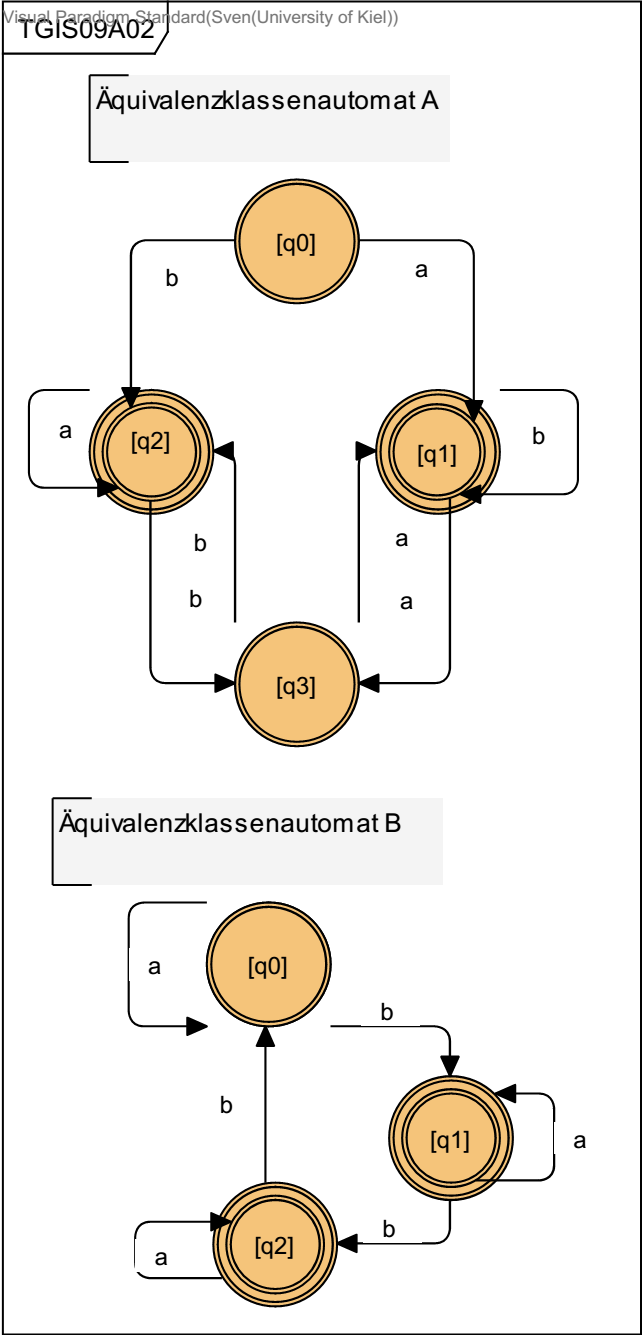
\includegraphics[scale=0.5]{part/TGIS09A02.png}

